\section{Density Estimation}


\mode<presentation>{
\begin{frame} 
    \begin{center} \huge
        \secname
    \end{center}
    %\begin{center} \large
        %\subsecname
    %\end{center}
	
\end{frame}
}

\subsection{What and Why?}

\begin{frame}{\secname:~\subsecname}

\notesonly{
We observe data. 
This data is generated by some unknown probability distribution. Each observation is a sample from this distribution.
When we talk about density estimation, we are talking about recovering the underlying probability density function that produced the observed samples.
}

\question{Why do we care about estimating densities? What can we do with an estimated density?}

\begin{itemize}
\item data exploration
\item visualization for 1D and 2D data (no dimensionality reduction)
\item deduce moments (mean, variance, \ldots)
\item describe the data in compact form (e.g. ``this data follows a Gaussian with mean $\mu$ and variance $\sigma^2$'')
\item generate new data
\item unsupervised anomaly detection
\end{itemize}

\end{frame}

\subsection{Strategies}

\begin{frame}{\subsecname}

2 strategies:

\begin{enumerate}[(A)]
\item \textbf{parametric} methods:
\\ We assume that the data follows some class of distribution and we estimate its parameters (e.g. fit a Gaussian around this data)
\item \textbf{non-parametric}\footnote{non-parametric does not means it is void of parameters. 
It is just that the parameters do not directly correspond to the classical parameters of densities such as mean and variance.} methods: 
data-driven. Estimate the density with as few assumptions as possible (e.g. Kernel\footnote{Not tied to Mercer Kernels like in Kernel PCA. A kernel is just some non-negative function.} density estimation)
\end{enumerate}

\end{frame}

\begin{frame}
\only<1>{\frametitle{Histograms}}
\only<2>{\frametitle{Normalized Histograms $\rightarrow$ density}}

\notesonly{
Many people have already encountered density estimation in the form of histograms.
}

\begin{minipage}{0.48\textwidth}
\begin{center}
	\includegraphics<1->[width=0.95\textwidth]{./img/hist}
	\notesonly{\captionof{figure}{Example histogram}}
\end{center}
\end{minipage}
\begin{minipage}{0.48\textwidth}
\begin{center}
	\includegraphics<2>[width=0.95\textwidth]{./img/hist_density}
	\notesonly{\captionof{figure}{Example density using a normalized histogram}}
\end{center}
\end{minipage}

\end{frame}

\subsection{Kernel density estimation (KDE)}

\mode<presentation>{
\begin{frame} 
    \begin{center} \huge
        \subsecname
    \end{center}
    \begin{center}
        Data-driven ``histogram bin placement''
    \end{center}
	
\end{frame}
}

\begin{frame}{\subsecname}
	
\begin{center}
	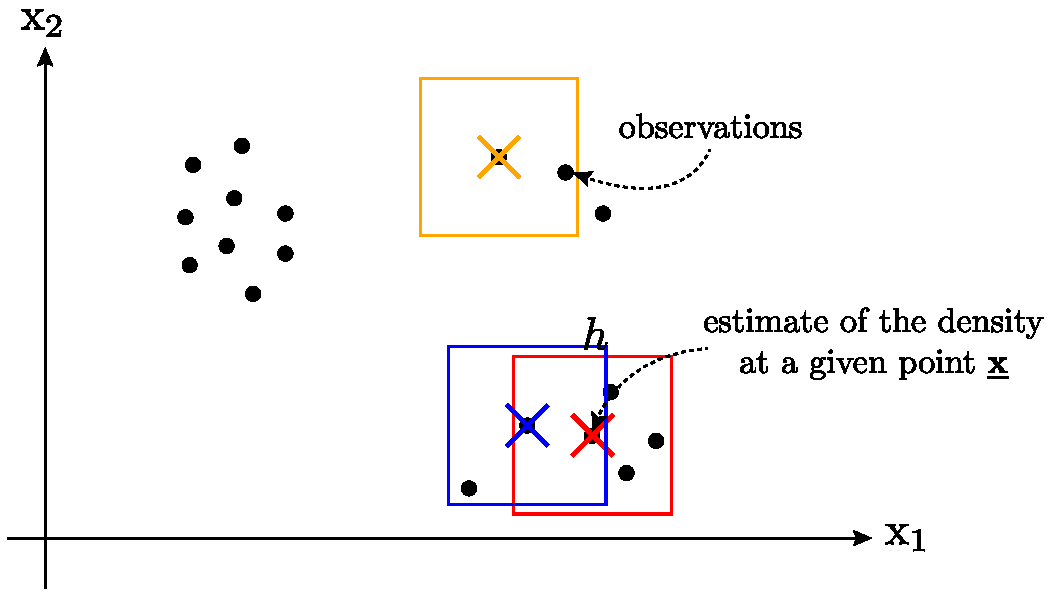
\includegraphics[width=0.6\textwidth]{./img/section1_fig1}
	\notesonly{\captionof{figure}{Kernel density estimation}}
\end{center}

Count the number of data points within a volume $V$ centered on $\vec{x}$.
Normalize to turn into a density estimate $\widehat{P}(\vec{x})$.

\end{frame}

\begin{frame}[t]{``Gliding histograms'' -- 1D case}
\small
\vspace{-0.3cm}
\slidesonly{Count the number of data points within a volume $V$ centered on $\vec{x}$.\\\vspace{0.1cm}}
Histogram kernel:
\begin{equation*}
\begin{array}{ll}
H({u}) = \left \{ \begin{array}{ll}
1, & u \in (-\frac{1}{2}, \frac{1}{2}) \\\\
0, & \text{else}
\end{array} \right.
\end{array}
\end{equation*}
Density estimate (``gliding histogram''):
\vspace{-0.3cm}
\begin{equation*}
	\widehat{P}({x};h) = 
	 \kern-3ex \underbrace{ \frac{1}{h}}_{
	\substack{ \text{normalization}}}
	 \kern-1.5ex 
\cdot \underbrace{ \frac{1}{p} 
	\overbrace{ \sum\limits_{\alpha = 1}^p
		H \bigg( \frac{{x} - {x}^{(\alpha)}}{
			h} \bigg) }^{
		\substack{\text{number of data points}\\
			\text{within window } (x-\frac{1}{2}, x+\frac{1}{2}) \\
			\text{ around } {x}}} }_{
	\text{fraction of data points}}
\end{equation*}
Histogram kernels lead to discontinuous pdf estimates $\leadsto$ use other kernels for smooth pdf estimates. 
\end{frame}


\begin{frame}[t]{``Gliding histograms'' -- N-dim data}
\small
Let $\vec x \in \R^N$:\\
%\vspace{-0.3cm}
\slidesonly{Count the number of data points within a volume $V$ centered on $\vec{x}$.\\\vspace{0.1cm}}
Histogram kernel:
\begin{equation*}
\begin{array}{ll}
H(\vec{u}) = \left \{ \begin{array}{ll}
1, & |u_j| < \frac{1}{2}, \forall j \in 1, \ldots, N \\\\
0, & \text{else}
\end{array} \right.
\end{array}
\end{equation*}
Density estimate (``gliding histogram''):
\vspace{-0.3cm}
\begin{equation*}
	\widehat{P}(\vec{x}) = \kern-3ex \underbrace{ \frac{1}{h^N} }_{
	\substack{ \text{normalization} \\
		\text{(``density''!)}}}
		\kern-1ex
\cdot \underbrace{ \frac{1}{p} 
	\overbrace{ \sum\limits_{\alpha = 1}^p
		H \bigg( \frac{\vec{x} - \vec{x}^{(\alpha)}}{
			h} \bigg) }^{
		\substack{\text{number of data points}\\
			\text{within volume } V 
			\text{ around } \vec{x}}} }_{
	\text{fraction of data points}}
\end{equation*}
Histogram kernels lead to discontinuous pdf estimates $\leadsto$ use other kernels for smooth pdf estimates. 
\end{frame}

\begin{frame}{Kernels}

\begin{center}	
	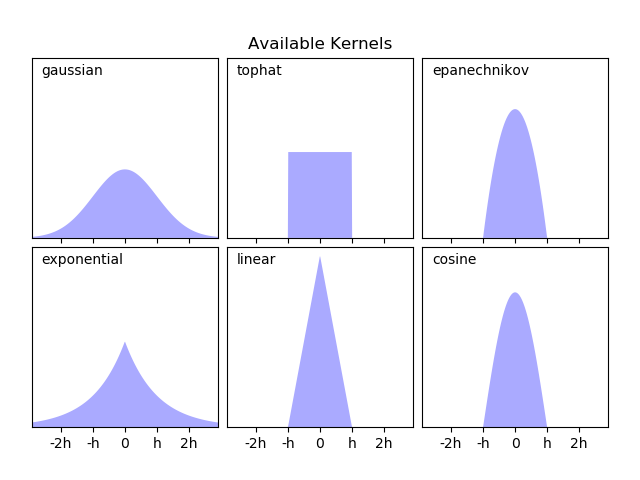
\includegraphics[width=0.6\textwidth]{./img/sphx_glr_plot_kde_1d_0021}
	\notesonly{\captionof{figure}{Kernel functions}}
\end{center}

{\footnotesize
Figure from https://scikit-learn.org/stable/modules/density.html
}


\end{frame}

\begin{frame}{Histogram vs. KDE}

\svspace{-3mm}

\begin{center}	
	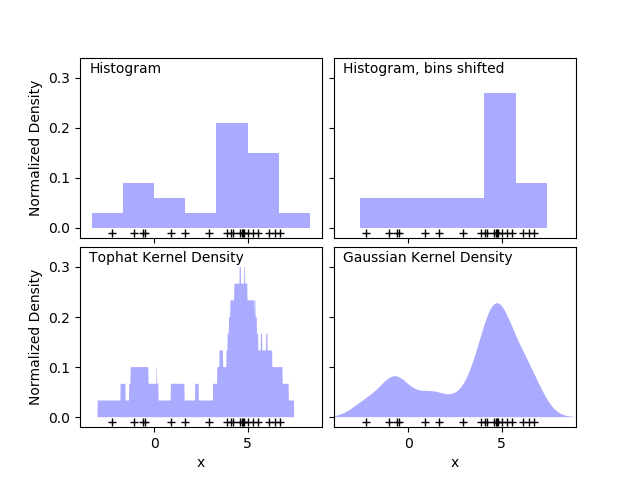
\includegraphics[width=0.5\textwidth]{./img/sphx_glr_plot_kde_1d_0011}
	\notesonly{\captionof{figure}{Histograms vs. KDE using different kernel functions}}
\end{center}

\svspace{-3mm}

Gaussian Kernel (1D case):

\svspace{-3mm}

\begin{equation}
H(u) = \frac{1}{\sqrt{2\pi}} \exp\Big({\frac{-u^2}{2}}\Big)
\end{equation}

\begin{equation}
\widehat{P}({x}, h) = \frac{1}{h p \sqrt{2\pi}} \sum_{\alpha=1}^p \exp \Big\{ -\frac{(x-x^{(\alpha)})^2}{2h^2} \Big\}
\end{equation}

{\footnotesize
Figure from https://scikit-learn.org/stable/modules/density.html
}

\end{frame}

\subsubsection{Choice of kernel width}


\begin{frame}{\subsubsecname}

\begin{figure}
	\centering
	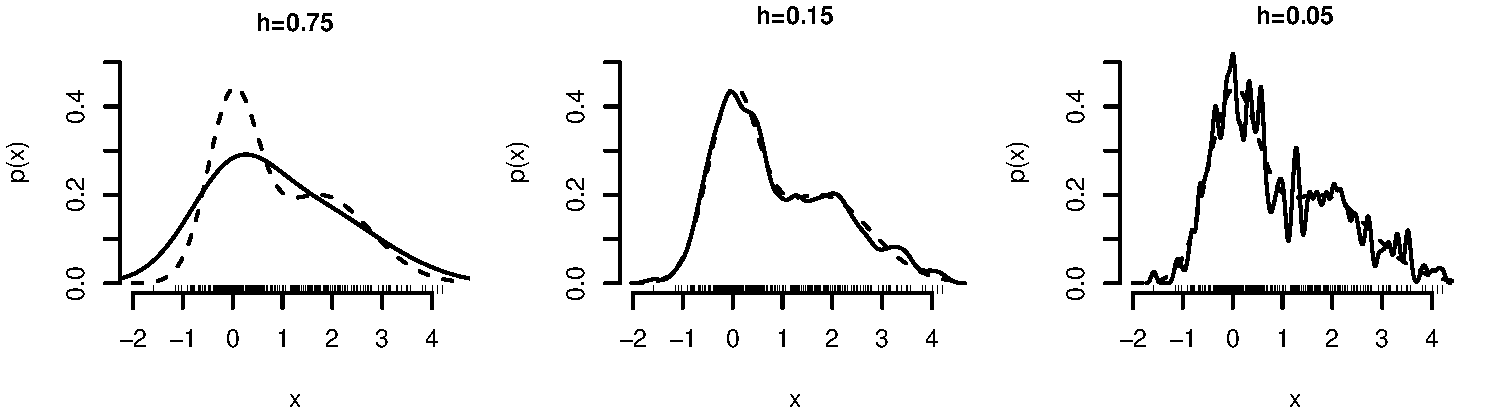
\includegraphics[width=\textwidth]{img/densExamples.pdf}\
	\notesonly{\captionof{figure}{Effect of kernel width h}}
\end{figure}

Choice of kernel width $h > 0$ $\Rightarrow$ model selection / validation


\end{frame}
